\section{AU2}
Text

\subsection{BDD}
Text

\begin{figure}[H]
	\centering
	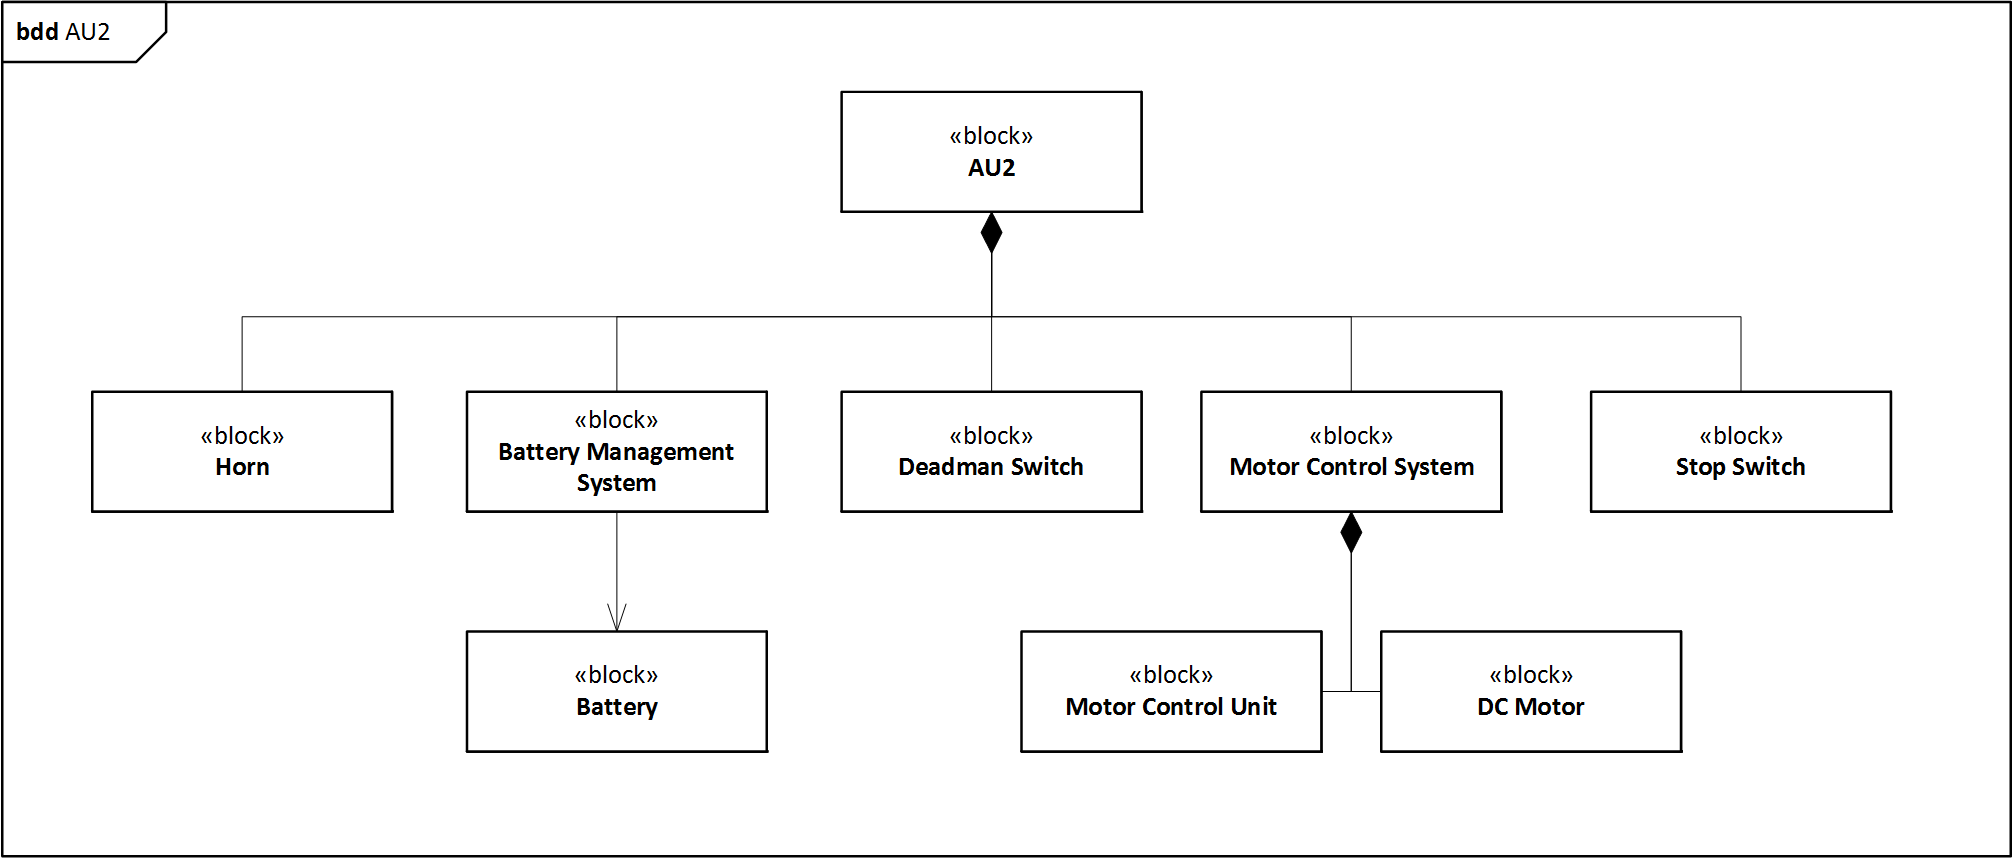
\includegraphics[width=0.9\linewidth]{Architecture/BDD_AU2}
	\caption{ BDD for AU2}
	\label{fig:AU2_BDD}
\end{figure}

\subsection{IBD}
Text

\begin{figure}[H]
	\centering
	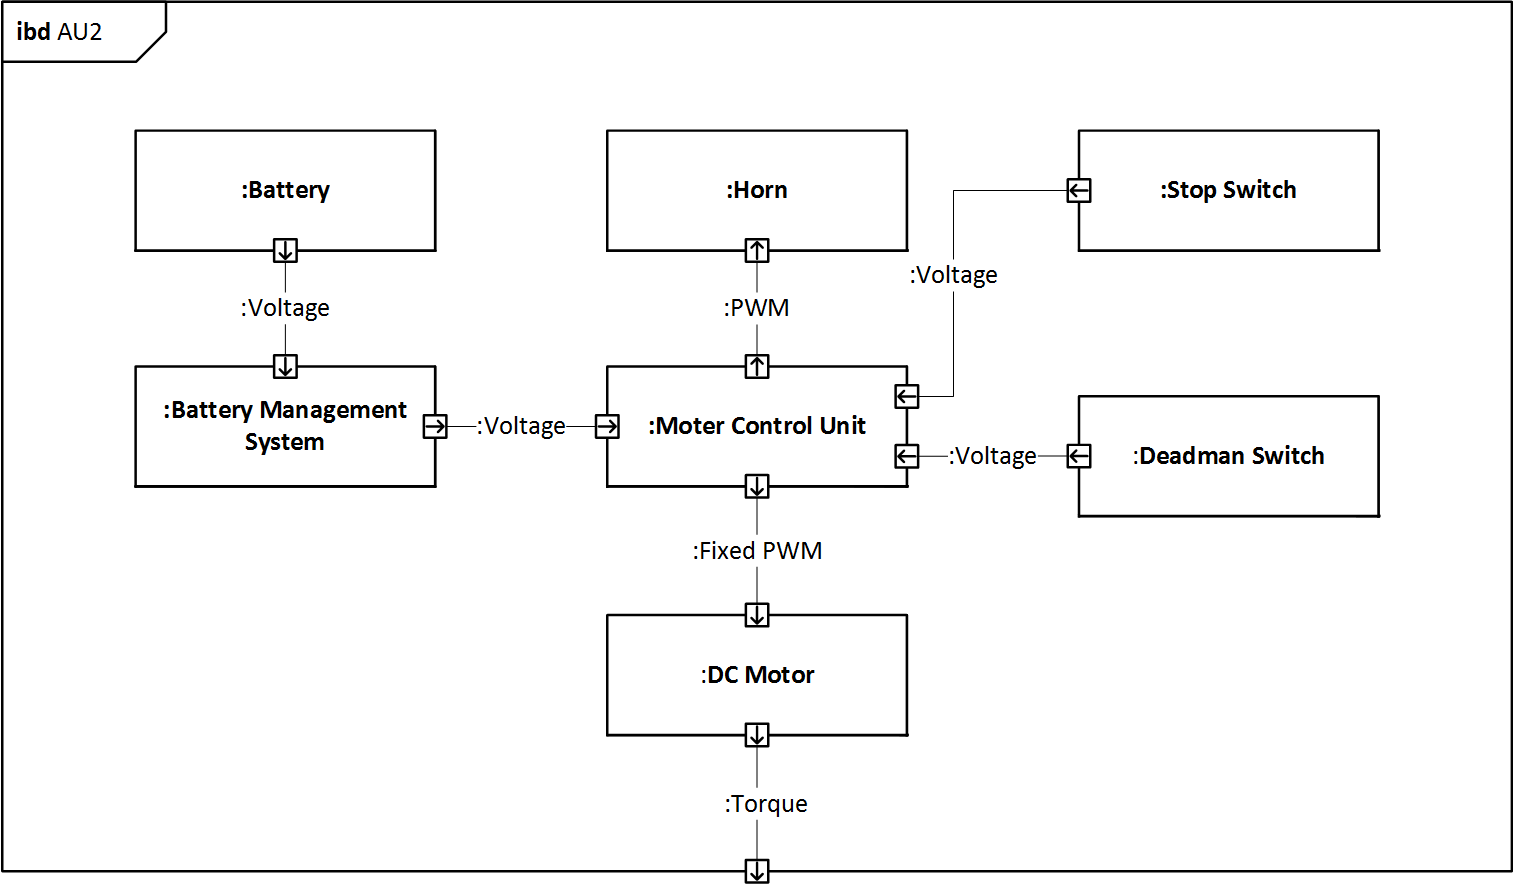
\includegraphics[width=0.9\linewidth]{Architecture/IBD_AU2}
	\caption{IBD for AU2}
	\label{fig:AU2_IBD}
\end{figure}

\subsection{Signal description}
The signals and protocols used to communicate between the blocks in AU2 are specified in this section.

\textbf{Block :Battery}\\
The battery transmits power to the Battery Management System.\\Interface description:

\begin{itemize}
	\item \textbf{:Power}\\
		Direction: [Battery] $\rightarrow$ [Battery Management System]\\
		Description: The supplied power from the Battery.
\end{itemize}

\textbf{Block :Battery Management System}\\
The power transmitted from the Battery is distributed to Motor Control Unit and DC Motor.\\
Interface description:

\begin{itemize}
	\item \textbf{CU :Power}\\
		Direction: [Battery Management System] $\rightarrow$ [Motor Control Unit]\\
		Description: The distributed power from the Battery Management System to the Motor Control Unit.
	\item \textbf{DC\_Motor :Power}
		Direction: [Battery Management System] $\rightarrow$ [DC Motor]\\
		Description: The distributed power from the Battery Management System to the DC Motor.
\end{itemize}

\textbf{Block :Horn}\\
The Horn receives a PWM signal from the Motor Control Unit when the Horn should sound and with a frequency represented as the frequency of the sound.\\
Interface description:

\begin{itemize}
	\item \textbf{:Power}\\
		Diretion: [Motor Control Unit] $\rightarrow$ [Horn]\\
		Description: The PWM signal from the Motor Control Unit to the Horn, which controls the frequency of the sound.
\end{itemize}

\textbf{Block :DC Motor}
The DC Motor receives the distributed power from the Battery Management System. Furthermore receives the DC Motor a PWM signal from the Motor Control Unit when the DC Motor must speed up, and a duty cycle on zero when the DC Motor must coast.\\
Interface description:

\begin{itemize}
	\item \textbf{:Fixed PWM}\\
		Direction: [Motor Control Unit] $\rightarrow$ [DC Motor]\\
		Description: The PWM signal from the Motor Control Unit is at a fixed PWM duty cycle when the DC Motor must speed up. When the DC Motor is coasting the PWM duty cycle becomes zero.
	\item \textbf{DC\_Motor :Power}\\
		Direction: [Battery Management System] $\rightarrow$ [DC Motor]\\
		Description: The distributed power from the Battery Management System to the DC Motor.
	\item \textbf{:Torque}\\
		Direction: [DC Motor] $\rightarrow$ [External Car Wheel]\\
		The Torque from the DC Motor to the External Car Wheel.
\end{itemize}

\textbf{Block :Stop Switch}\\
The Stop Switch transmits a “high” XXX\fxnote{uddyb signalbeskrivelse} Voltage to the Motor Control Unit when the Stop Switch is pressed and thereby closed. A “low” XXX \fxnote{uddyb signalbeskrivelse, skal stemme overens med µC} Voltage is transmitted to the Motor Control Unit when the Stop Switch is open, which makes the car able to drive.\\
Interface description:

\begin{itemize}
	\item \textbf{:Voltage}\\
		Direction: [Stop Switch] $\rightarrow$ [Motor Control Unit]\\
		Description: A digital signal from the Stop Switch to the Motor Control Unit XXXX\fxnote{uddyb} Voltage. When the digital signal is “high” the car must stop, and when “low” the car must be able to drive.
\end{itemize}

\textbf{Block :Deadman Switch}\\
The Deadman Switch transmits a “high” XXXVoltage to the Motor Control Unit when the Deadman Switch is pressed. A “low” XXXVoltage is transmitted to the Motor Control Unit when the Stop Switch is open, which must stop the car.
Interface description:

\begin{itemize}
	\item \textbf{:Voltage}\\
		Direction: [Deadman Switch] $\rightarrow$ [Motor Control Unit]\\
		Description: A digital signal from the Deadman Switch to the Motor Control Unit XXXXVoltage. When the digital signal is “high” the car must be able to drive, and when “low” the car must stop.
\end{itemize}

\textbf{Block :Motor Control Unit}\\
The Motor Control Unit controls the DC Motor and the Horn with PWM signals. The Motor Control Unit receives power from the Battery Management System, a digital signal from the Stop Switch and a digital signal from the Deadman Switch.\\
Interface description:

\begin{itemize}
	\item \textbf{CU :Power}\\
		Direction: [Battery Management System] $\rightarrow$ [Motor Control Unit]\\
		Description: The distributed power from the Battery Management System to the Motor Control Unit.
	\item \textbf{:Power}\\
		Direction: [Motor Control Unit] $\rightarrow$ [Horn]\\
		Description: The PWM signal from the Motor Control Unit to the Horn, which controls the frequency of the sound.
	\item \textbf{:Fixed PWM}\\
		Direction: [Motor Control Unit] $\rightarrow$ [DC Motor]\\
		Description: The PWM signal from the Motor Control Unit is at a fixed PWM duty cycle when the DC Motor must speed up. When the DC Motor is coasting the PWM duty cycle becomes zero.
	\item \textbf{:Voltage}\\
		Direction: [Stop Switch] $\rightarrow$ [Motor Control Unit]\\
		Description: A digital signal from the Stop Switch to the Motor Control Unit XXXXVoltage. When the digital signal is “high” the car must stop, and when “low” the car must be able to drive.
	\item \textbf{:Voltage}\\
		Direction: [Deadman Switch] $\rightarrow$ [Motor Control Unit]\\
		Description: A digital signal from the Deadman Switch to the Motor Control Unit XXXXVoltage. When the digital signal is “high” the car must be able to drive, and when “low” the car must stop.
\end{itemize}